\chapter{Statistical Testing of GP-EKF}\label{chap:stat_testing}
Inspired by \cite{hexeberg}, we will test the performance of the model for straight-line trajectories and curved trajectories independently.

\section{Metrics}
\subsection{Trajectory Error}
The trajectory error is found by comparing the predicted position with the ground truth. As the predicted trajectory is simulated in discrete time, the points with the closest timestamps are used for comparison. With $\Delta T = 10\text{ seconds}$, the maximum error in time is $\frac{\Delta T}{2} = 5 \text{ seconds}$, which is considered to be acceptable considering the time-horizon of between $15$ and $30$ minutes. 
\subsection{Path Error}
The path error is defined as the closest point in the predicted trajectory to each point in the ground truth, under the constraint that the corresponding predicted timestamps must be monotonically increasing. In other words, the path cannot move backward in time. Linear interpolation is used to get the path error at fixed timestamps to simplify the comparison. 

\subsection{Interpolation}
Linear interpolation is used to compare the error at fixed timestamps between samples. The error for short trajectories is not extrapolated.

\section{Straigth-line trajectories}
We use the first $100$ randomly sampled trajectories satisfying the following requirements:
\begin{enumerate}
    \item The sum of subsequent changes in \acrshort{cog} must be less than $30$ degrees, i.e., the trajectory must be close to a straight line.
    \item There must be sufficient data available for training in the neighborhood around the initial starting point, with similar initial heading and speed.
\end{enumerate}

\begin{table}[h]
    \begin{subtable}{\textwidth}
        \makebox[\textwidth][c]{
            \begin{tabular}{lllrrrrr}
                \toprule
                        &                & Time [Minutes]    & 5   & 10   & 15   & 20   & 25   \\
                Summary & Method         & Training Source   &     &      &      &      &      \\
                \midrule
                Mean    & CVM            & COG/SOG from AIS  & 582 & 1163 & 1794 & 2053 & 2836 \\
                        & GP-EKF         & COG/SOG from AIS  & 552 & 1053 & 1533 & 1976 & 1898 \\
                        &                & Finite Difference & 547 & 1006 & 1524 & 2282 & 1945 \\
                        & GP-EKF w/ PDAF & COG/SOG from AIS  & 554 & 1047 & 1529 & 2013 & 1875 \\
                        &                & Finite Difference & 535 & 978  & 1476 & 2258 & 1990 \\
                \midrule
                Median  & CVM            & COG/SOG from AIS  & 445 & 870  & 1367 & 1734 & 2170 \\
                        & GP-EKF         & COG/SOG from AIS  & 477 & 904  & 1285 & 1585 & 1585 \\
                        &                & Finite Difference & 455 & 787  & 1142 & 1616 & 1352 \\
                        & GP-EKF w/ PDAF & COG/SOG from AIS  & 475 & 877  & 1243 & 1561 & 1429 \\
                        &                & Finite Difference & 427 & 744  & 1076 & 1474 & 1638 \\
                %\bottomrule
            \end{tabular}
        }
        \caption{Trajectory errors in meters}
        \label{table:stats_straight_traj_err}
        \vspace*{0.5cm}
    \end{subtable}
    \begin{subtable}{\textwidth}
        \makebox[\textwidth][c]{
            \begin{tabular}{lllrrrrr}
                \toprule
                        &                & Time [Minutes]    & 5   & 10  & 15   & 20   & 25   \\
                Summary & Method         & Training Source   &     &     &      &      &      \\
                \midrule
                Mean    & CVM            & COG/SOG from AIS  & 122 & 414 & 1004 & 1383 & 1872 \\
                        & GP-EKF         & COG/SOG from AIS  & 216 & 422 & 843  & 1230 & 1091 \\
                        &                & Finite Difference & 234 & 446 & 717  & 1226 & 782  \\
                        & GP-EKF w/ PDAF & COG/SOG from AIS  & 206 & 401 & 822  & 1249 & 1107 \\
                        &                & Finite Difference & 223 & 414 & 673  & 1223 & 871  \\
                \midrule
                Median  & CVM            & COG/SOG from AIS  & 61  & 197 & 553  & 1001 & 1564 \\
                        & GP-EKF         & COG/SOG from AIS  & 147 & 283 & 517  & 815  & 731  \\
                        &                & Finite Difference & 151 & 273 & 399  & 559  & 625  \\
                        & GP-EKF w/ PDAF & COG/SOG from AIS  & 149 & 270 & 534  & 851  & 728  \\
                        &                & Finite Difference & 152 & 273 & 383  & 609  & 633  \\
                \bottomrule
            \end{tabular}
        }
        \caption{Path error in meters}
        \label{table:stats_straight_path_err}
    \end{subtable}
    \caption{Error summary for $350$ straight-line trajectories. Mean and median summary statistics are calculated for the trajectory and path error at fixed timestamps. Linear interpolation is used between samples. Errors for short trajectories are not extrapolated, and therefore not included in the $20$ and $25$ minute bins.}
    \label{table:stats_straigh_line_error}
\end{table}



\section{Curved Trajectories}
We use the first $100$ randomly sampled trajectories satisfying the following requirements:
\begin{enumerate}
    \item The sum of subsequent changes in \acrshort{cog} must be greater than $40$ degrees, i.e., the trajectory must be close to a straight line.
    \item There must be sufficient data available for training in the neighborhood around the initial starting point, with similar initial heading and speed.
\end{enumerate}

\begin{table}[h]
    \begin{subtable}{\textwidth}
        \makebox[\textwidth][c]{
            \begin{tabular}{lllrrrrr}
                \toprule
                        &                & Time [Minutes]    & 5    & 10   & 15   & 20   & 25    \\
                Summary & Method         & Training Source   &      &      &      &      &       \\
                \midrule
                Mean    & CVM            & COG/SOG from AIS  & 1451 & 3492 & 6354 & 9925 & 17156 \\
                        & GP-EKF         & COG/SOG from AIS  & 806  & 1674 & 2437 & 2838 & 3879  \\
                        &                & Finite Difference & 656  & 1356 & 1850 & 2273 & 2371  \\
                        & GP-EKF w/ PDAF & COG/SOG from AIS  & 749  & 1532 & 2165 & 2358 & 3003  \\
                        &                & Finite Difference & 664  & 1312 & 1776 & 2166 & 2240  \\
                \midrule
                Median  & CVM            & COG/SOG from AIS  & 952  & 2515 & 4828 & 8597 & 14719 \\
                        & GP-EKF         & COG/SOG from AIS  & 648  & 1311 & 1931 & 2412 & 3275  \\
                        &                & Finite Difference & 457  & 931  & 1369 & 1873 & 1784  \\
                        & GP-EKF w/ PDAF & COG/SOG from AIS  & 574  & 1117 & 1513 & 1697 & 2016  \\
                        &                & Finite Difference & 480  & 881  & 1323 & 1719 & 1654  \\
                \bottomrule
            \end{tabular}
        }
        \caption{Trajectory Error in meters}
        \label{table:stats_curved_traj_err}
        \vspace*{0.5cm}
    \end{subtable}
    \begin{subtable}{\textwidth}
        \makebox[\textwidth][c]{
            \begin{tabular}{lllrrrrr}
                \toprule
                        &                & Time [Minutes]    & 5   & 10   & 15   & 20   & 25   \\
                Summary & Method         & Training Source   &     &      &      &      &      \\
                \midrule
                Mean    & CVM            & COG/SOG from AIS  & 562 & 1458 & 2929 & 4149 & 6466 \\
                        & GP-EKF         & COG/SOG from AIS  & 312 & 737  & 1465 & 1986 & 3010 \\
                        &                & Finite Difference & 369 & 605  & 747  & 730  & 605  \\
                        & GP-EKF w/ PDAF & COG/SOG from AIS  & 285 & 616  & 1190 & 1485 & 2172 \\
                        &                & Finite Difference & 366 & 569  & 693  & 687  & 593  \\
                \midrule
                Median  & CVM            & COG/SOG from AIS  & 188 & 856  & 1967 & 3405 & 5524 \\
                        & GP-EKF         & COG/SOG from AIS  & 141 & 328  & 982  & 1388 & 2621 \\
                        &                & Finite Difference & 203 & 398  & 447  & 435  & 376  \\
                        & GP-EKF w/ PDAF & COG/SOG from AIS  & 133 & 248  & 643  & 866  & 1347 \\
                        &                & Finite Difference & 220 & 393  & 429  & 405  & 373  \\
                \bottomrule
            \end{tabular}
        }
        \caption{Path error in meters}
        \label{table:stats_curved_path_err}
    \end{subtable}
    \caption{Error summary for $350$ curved trajectories. Mean and median summary statistics are calculated for the trajectory and path error at fixed timestamps. Linear interpolation is used between samples. Errors for short trajectories are not extrapolated, and therefore not included in the $20$ and $25$ minute bins.}
    \label{table:stats_curved_error}
\end{table}

\section{Comparing GP-EKF to CVM}
As expected, the CVM method struggles with curved trajectories, leading to large trajectory errors. The GP-EKF approach performs significantly better, with overall lower spread and median trajectory error as depicted in \cref{fig:stats_curved_gp_ekf_cvm}.
\begin{figure}[h]
    \centering
    \makebox[\textwidth][c]{
        \begin{subfigure}{0.65\textwidth}
            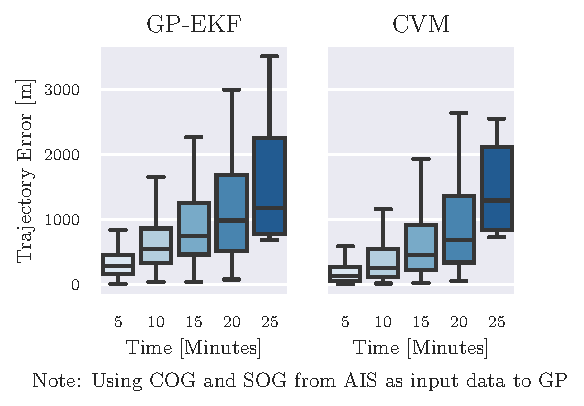
\includegraphics[width=\textwidth]{figures/straight_line_stats/gp_vs_cvm_2.pdf}
            \caption{Straight-Line Trajectories}
        \end{subfigure}
        \begin{subfigure}{0.65\textwidth}
            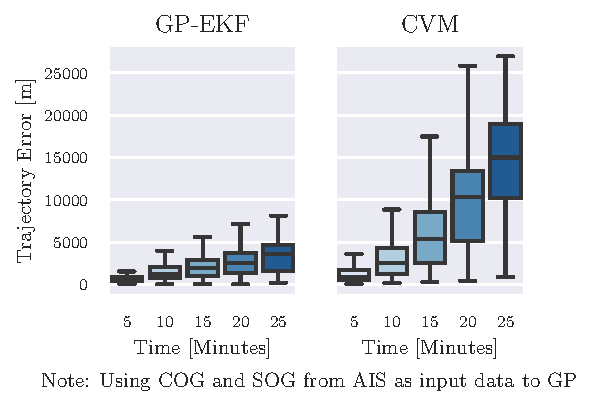
\includegraphics[width=\textwidth]{figures/curved_line_stats/gp_vs_cvm_2.pdf}
            \caption{Curved Trajectories}
        \end{subfigure}
    }
    \caption{GP-EKF compared to the CVM method on $350$ random trajectories. As expected, the \acrshort{cvm} yields large trajectory errors on curved trajectories. The GP-EKF performs consistently better, with lower median error as well as lower spread. However, on straight-line trajectories, the methods behave comparably.}
    \label{fig:stats_curved_gp_ekf_cvm}
\end{figure}

\section{Effect of the PDAF update}
\begin{figure}[h]
    \centering
    \makebox[\textwidth][c]{
        \begin{subfigure}{0.65\textwidth}
            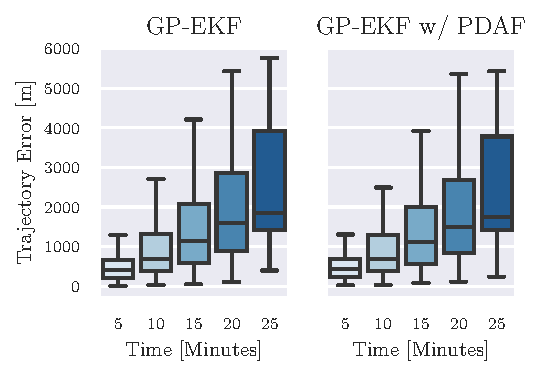
\includegraphics[width=\textwidth]{figures/straight_line_stats/gp_vs_pdaf.pdf}
            \caption{Straight-Line Trajectories}
        \end{subfigure}
        \begin{subfigure}{0.65\textwidth}
            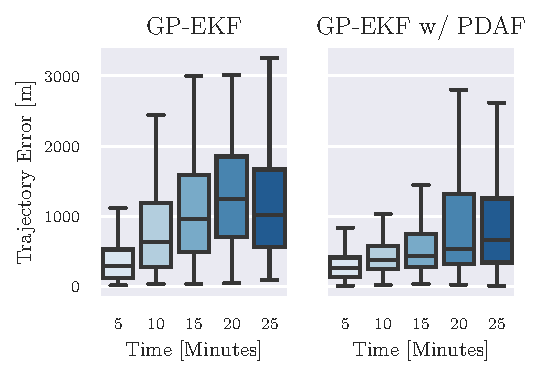
\includegraphics[width=\textwidth]{figures/curved_line_stats/gp_vs_pdaf.pdf}
            \caption{Curved Trajectories}
        \end{subfigure}
    }
    \caption{GP-EKF with and without PDAF on curved trajectories for $350$ trajectories. While there are some slight differences, the \acrshort{pdaf} does not appear to have any considerable effect on the trajectory errors.}
    \label{fig:stats_curved_gp_ekf_with_or_without_pdaf}
\end{figure}

\section{Finite Difference vs. COG/SOG from AIS}
A key design choice for the GP-EKF is which data source to use for training. The model can either be trained using the \acrshort{cog} and \acrshort{sog} values contained in the \acrshort{ais} samples or by calculating numerical derivatives of the position through a finite-difference approach. Comparing trajectory error for both approaches on the same test set favors the finite-difference approach, as seen in \cref{fig:stats_curved_gp_ekf_fd_vs_cog}. The finite difference approach performs consistently better, with lower median error and less spread. However, by ignoring the time component, looking at the path errors in \cref{table:stats_curved_path_err} supports the opposite, where the path errors are lower for the \acrshort{cog}/\acrshort{sog} approach. This may indicate that the issue is due to imprecise velocity estimates from the \acrshort{sog} while using the course from the \acrshort{cog} works well.
\begin{figure}[h]
    \centering
    \makebox[\textwidth][c]{
        \begin{subfigure}{0.65\textwidth}
            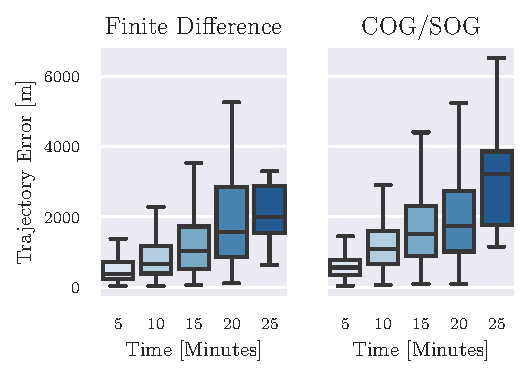
\includegraphics{figures/straight_line_stats/gp_cog_vs_fd.pdf}
            \caption{Straight-Line Trajectory}
        \end{subfigure}
        \begin{subfigure}{0.65\textwidth}
            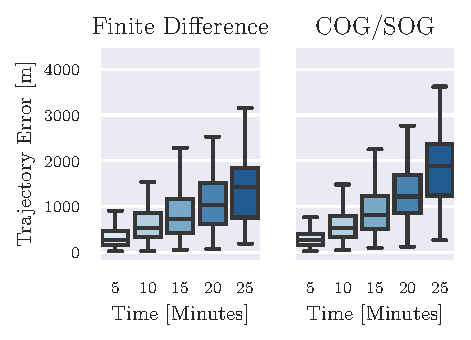
\includegraphics{figures/curved_line_stats/gp_cog_vs_fd.pdf}
            \caption{Curved Trajectory}
        \end{subfigure}
    }
    \caption{GP-EKF using finite differences and the \acrshort{cog} and \acrshort{sog} from the AIS dataset on $350$ trajectories. The finite differences approach performs consistently better, with lower median error and spread.}
    \label{fig:stats_curved_gp_ekf_fd_vs_cog}
\end{figure}




\section{Consistency}
Insert plot of NEES here


